\clearpage
\subsection{Находим коэффициенты для системы с фазовой траекторией типа <<неустойчивый фокус>>}
. В качестве второй неустойчивой структуры примем структуру с фазовыми траекториями типа <<неустойчивый фокус>> ,то есть, раскручивающиеся спирали. Для получения такой фазовой траектории необходимо, чтобы корни характеристического  уравнения были комплексными сопряженными с положительными вещественными частями. Такую структуру можно получить за счёт соответствующего подбора коэффициентов в регуляторе. Приведенный ХП замкнутой системы  \eqref{eq:HP_2_por_upr1}был получен ранее. 
\begin{equation} \label{eq:HP_2_por_upr1}
D(p)=p^2+\left(\cfrac{k_{2}}{27}+\cfrac{4}{3}\right)\,p+\cfrac{k_{1}}{27}+\cfrac{1}{81}
\end{equation}

Для того, чтобы корни имели положительные вещественные части, необходимо, чтобы $\cfrac{k_{2}}{27}+\cfrac{4}{3}<0$, т.е. $k_2<-36$ .Знак минус у $k_2$  говорит о том, что обратная связь по производной от отклонения должна быть положительной, что в свою очередь объясняется тем, что сам объект является асимптотически устойчивым.Чтобы корни были комплексно-сопряженными необходимо выполнение  \eqref{eq:usl_ks}
\begin{equation} \label{eq:usl_ks}
k_1>\cfrac{{k_{2}}^2}{108}+\cfrac{2\,k_{2}}{3}+\cfrac{35}{3}
\end{equation}
Пусть $k_2=-72.00$

Тогда соответственно получаем $k_1>
11.7
$ и рассчитываем коэффициент $k_1$ : \begin{equation} \label{eq:}
k_1=100\times11.7=1.17e+03
\end{equation}

Корни характеристического полинома:
\begin{equation}p_1=
0.667-6.54i
\end{equation}
\begin{equation}p_2=
0.667+6.54i
\end{equation}

Схема будет иметь тот же вид, что и на рис.\ref{fig:sim_linear_2_por}.
Исследуем движение фазовых координат во времени посредством моделирования процессов в системе при отклонении системы от состояния равновесия. Фазовые траектории в системе на рис.\ref{fig:linear_2_por_ft_focus}. 
В дополнение на рис.\ref{fig:linear_2_por_sv_focus} указано изменение выходной переменной и её производной. 
\begin{figure}[!h]\centering
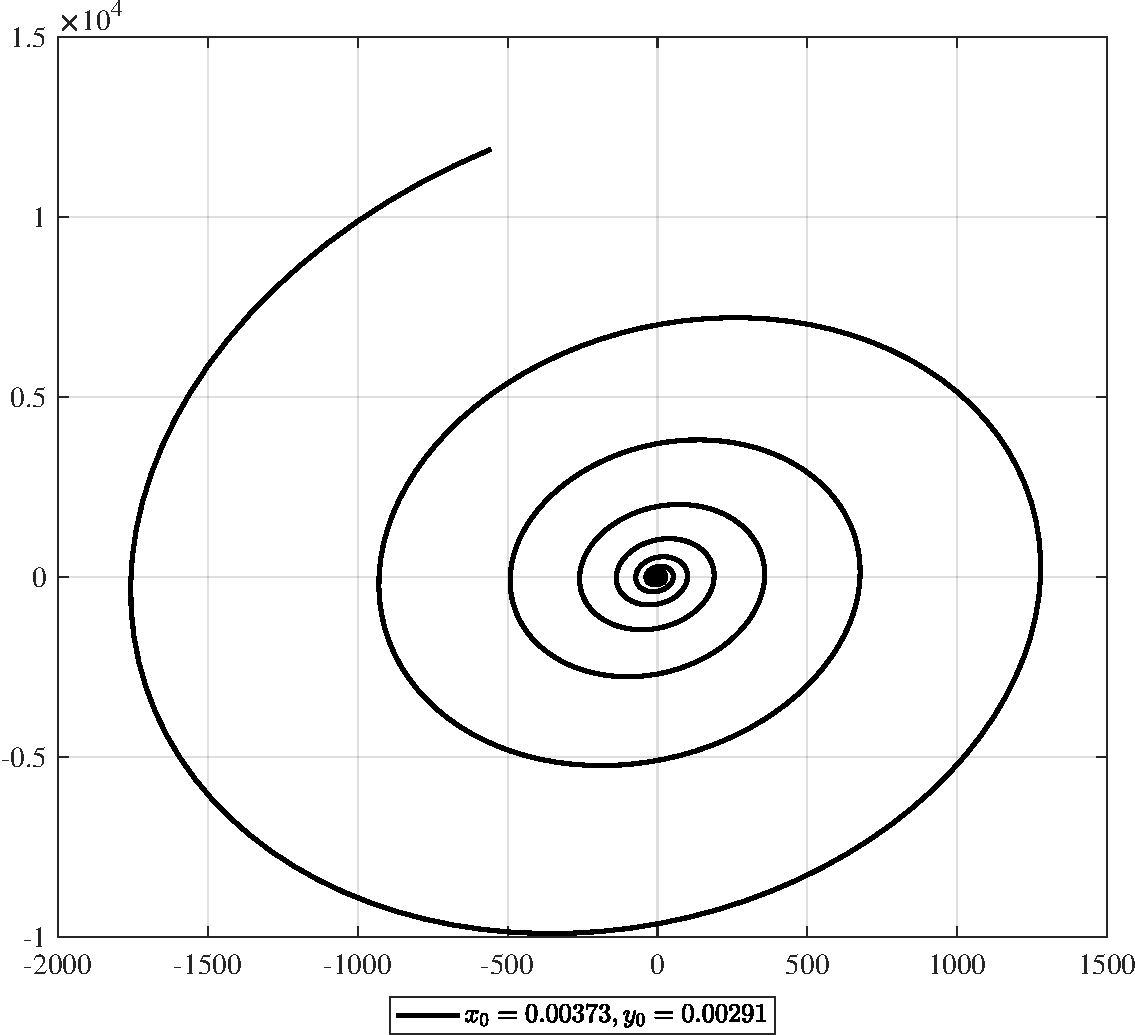
\includegraphics[width=1.0\linewidth]{images/linear_2_por_ft_focus}
\caption{ Фазовые траектории для системы с переменной структурой с разными начальными условиями.}\label{fig:linear_2_por_ft_focus}
\end{figure}
\begin{figure}[!h]\centering
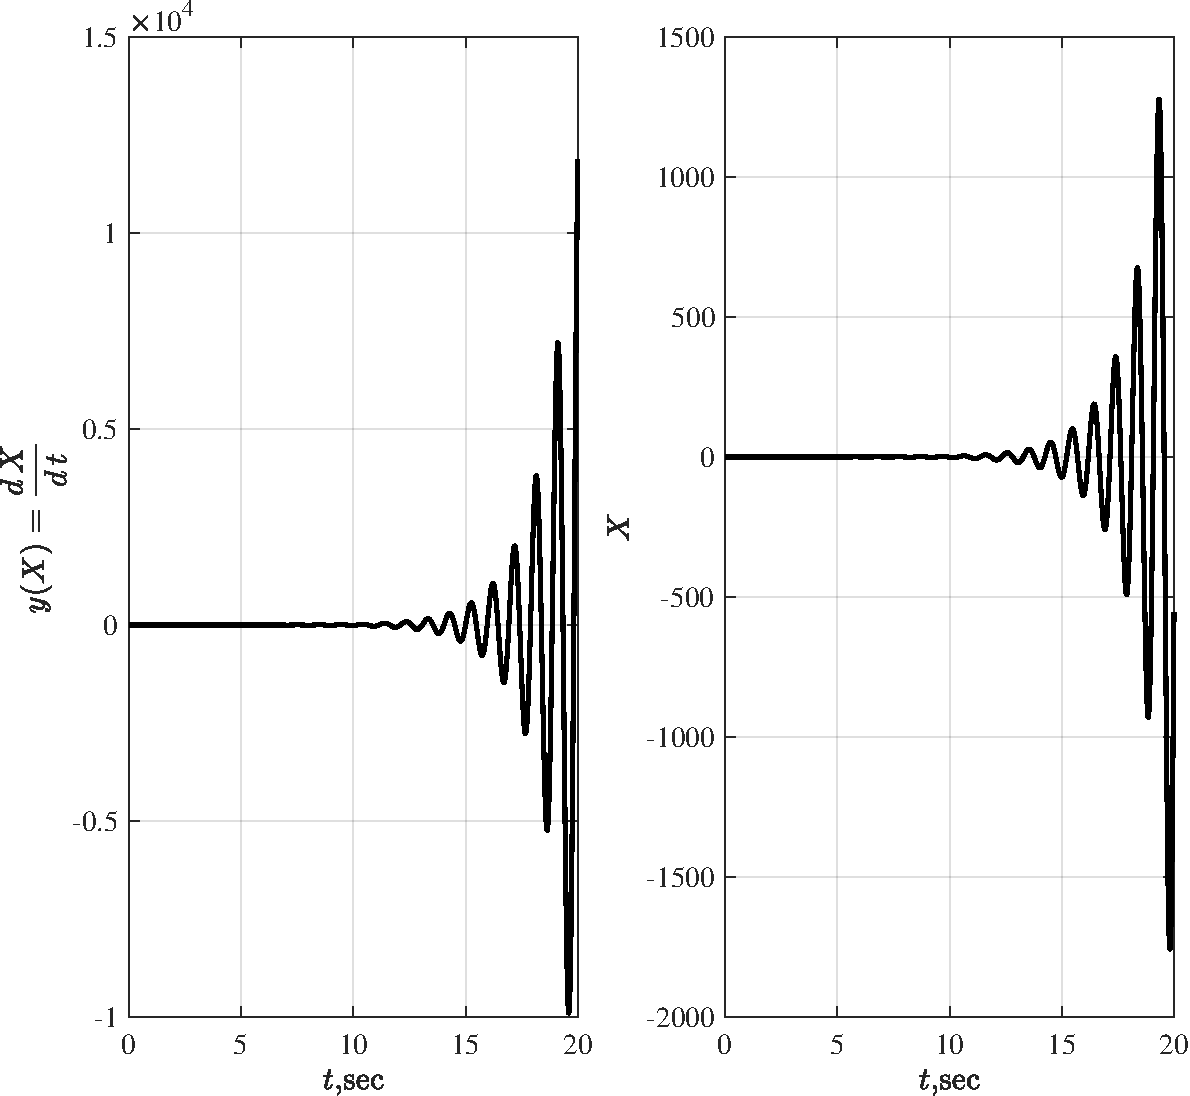
\includegraphics[width=1.0\linewidth]{images/linear_2_por_sv_focus}
\caption{ Графики изменения выходной переменной и её производной.}\label{fig:linear_2_por_sv_focus}
\end{figure}
